

\section{Opportunities of video}
\label{sec:video}



The ubiquity of Internet video opens new opportunities of network-wide traffic
and performance measurement.  The major advantage of Internet video lays in its
unprecedented coverage, both in space and time.  In this section, we present
early promise of the viability of video-based measurements to serve as the
basis for a real-time Internet traffic map.  We specifically focus on the {\em
coverage}  as observed over a  one-day period using data collected by a
third-party video analytics provider. The analytics provider runs a measurement
plugin that runs as part of several affiliate content providers' sites (who
span diverse content genres). This one-day dataset  contains 50~million
individual video sessions from 213 unique countries.
Table~\ref{tab:overview:statistics} shows the basic characteristics of the
dataset. 

\begin{table}[h!]
    \begin{tabular}{|l|l|}
    \hline
    Attributes      &  Possible values or \# of unique values                      \\ \hline
    CDN  & \shortstack{Akamai, Level3, Limelight, Amazon, \\Verizon, site-specific CDNs}   \\ \hline
    Site  &  379 \\ \hline
    AS        & 15K                \\ \hline
    ISP       &  170                \\ \hline
    City & 9700                 \\     \hline
    Country & 213                 \\    \hline
    \end{tabular}
\label{tab:overview:statistics}
\end{table}

Our focus in this section is on the {\em  temporal coverage}. \footnote{We
do not show the  spatial coverage  (e.g., the fraction of all ASes
in US covered by our dataset)as this inherently depends on how large 
  the provider collecting the data and thus reflects on the span of the provider more 
than the intrinsic characteristics of user arrivals.}
 For instance,  among all the ASes in
the dataset, what is the fraction that can be observed every 10 minute? This
indicates the finest time granularity that the video traffic offers to probe the
network. Specifically,   if an AS appears in every 1 minute, then a query pertinent 
 to that AS can potentially 
be answered based on measurements made within the last one minute. 
%\jc{somehow justify why we examine the edge coverage in terms of client-side
%and server-side}




%\begin{table}
%    \begin{tabular}{|l|ll|}
%    \hline
%    ~         & \# of unique ASes & \# of unique server IPes \\ \hline
%    Global    & 171              & 8376                    \\
%    US        & 75               & 6094                    \\
%    Akamai    & 140              & 2404                    \\
%    Level3    & 49               & 1299                    \\
%    Limelight & 2                & 191                     \\ \hline
%    \end{tabular}
%\tightcaption{Coverage on server side.}
%\end{table}

\subsection{Client-side coverage} 
Figure~\ref{fig:video:client-coverage} shows the temporal coverage in terms of client IP prefix (/24), AS, and ISP. For example, for AS (similar to IP prefix and ISP), we first chop the one-day period into windows of 1 minute (10 minutes or 1 hour), and then for each AS that has appeared at least once in the dataset, we calculate the fraction of windows in which the AS has at least 50 (almost) concurrent sessions. Finally, we plot its inverse CDF in Figure~\ref{fig:video:client-coverage}. 
It is shown that almost all ISPes (90\%) can be measured with very fine time granular (1 minute) while substantial fraction of /24 blocks (20\%), and ASes (36\%)  can be measured with very fine time granular (1 minute) as well. That means at any moment, it is possible to collect sufficient number of sessions from any ISP we manage to observe. Furthermore, it is shown that there is a significant improvement of using 10-minute window with respect to 1-minute window, which shows an explicit trade-off between high coverage and accuracy.


\subsection{Server-side coverage} 
Now, we use the server-side IP prefix (/24) to examine the server-side coverage, and use pair of IP prefix between server and client to show the coverage over client-server pairs. Similar to Figure~\ref{fig:video:client-coverage}, Figure~\ref{fig:video:server-coverage} shows the inverse CDF of fraction of windows in which each server or client-server pair can be measured. Note that inaccurate server IPs (e.g., 254.255.255.255) are filtered out. Again, a server IP prefix (same to client-server pair) has to appear in a window with enough sessions (more than 50).
It is shown that 55 \% of server IP prefix can be observed with enough sessions in every 1-minute windows. Coverage of client-server pair is lower with 40 \% of pairs being observed in at least 80 \% of 1-minute windows. It again shows a possible improvement by using 10-minute windows.


\begin{figure}[h!]
\centering
\subfigure[Server /24 prefix]
{
	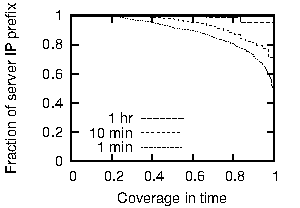
\includegraphics[width=140pt]{data2/serverPrefix-test-city.pdf}
}
\hspace{-0.5cm}
\subfigure[Pair of /24 prefix btw. client and server]
{
	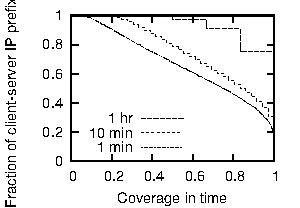
\includegraphics[width=140pt]{data2/cdf-test-asnServerPrefix.pdf}
}
\vspace{-0.1cm}
\tightcaption{Inverse CDF of server-side coverage (fraction of server-side IP prefix and server-client pairs which can be consistently measured) -- Above 55\% of observed server IP prefix and 20\% of server-client pairs can be measured in every minute. }
\label{fig:video:server-coverage}
\end{figure}

\begin{figure}[t!]
\centering
\subfigure[IP links]
{
	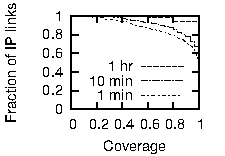
\includegraphics[width=120pt]{data2/cdf-test-link.pdf}
}
\hspace{-0.7cm}
%\subfigure[AS links (inter-domain links)]
%{
%	
\includegraphics[width=220pt]{figures/empty-figure.pdf}
%}
%\hspace{-0.5cm}
\subfigure[\# of concurrent sessions on each link]
{
	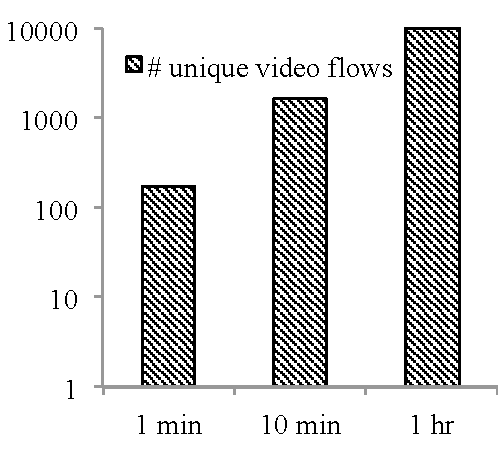
\includegraphics[width=110pt]{figures/link-load.pdf}
\label{fig:video:path-coverage-2}
}
\vspace{-0.3cm}
\tightcaption{Inverse CDF of fraction of IP links that can be consistently measured -- More than 60\% of observed links can be measured in every minute, with a median traffic volume of 170 unique video sessions in a one-minute time window.}
\label{fig:video:path-coverage}
\end{figure}

\subsection{Link coverage} Now we would like to investigate the coverage inside the network. Figure~\ref{fig:video:path-coverage} presents the inverse CDF of link coverage using the same methodology as in Figure~\ref{fig:video:client-coverage}. 
It is shown that more than 60 \% of observed links can be consistently probed in every minute. 
We also examine the traffic volume (i.e., number of current video sessions) we manage to measure on each link within different time granular. Figure~\ref{fig:video:path-coverage-2} shown that the median number of different current video sessions on each link during a time window of 1 minute, 10 minutes or one hour. The figure shows that each link will be probed every minute by 170 video sessions in median.

\subsection{Main observations}

In summary, we observe that by passively measuring the video traffic, 40 \% of
client-side AS can be measured with at least 50 simultaneous sessions in every
10 minutes and 36 \% of these can be even measured in every minutes. Moreover,
more than 30 \% of the paths from client IP prefix to server IP prefix in the
dataset is probed every 10 minutes with at least 50 simultaneous sessions.  



